\subsection*{Brief Recap\ldots}
Working with a real system
\begin{equation}
    (A + \delta A)x = b + \delta b 
\end{equation}

The numerical solution has some error $\delta x$, with bounds given
by

\begin{equation}
    \frac{\norm{\delta x}}{\norm{x}} \le \ldots
\end{equation}  

The larger the condition number, the closer it is to being a singular
matrice and inversion is numerically unstable. Geometrically, solving
$Ax = b$ is finding the intersection of planes. If the planes are
nearly parallel to each other, then even small deviations in the
planes will lead to large deviations in the intersection point.

\section*{Finite Precision Arithmetic}
Even if we know any quantity with infinite precision, we can only
store a representation of the quantity up to some finite precision.

The computers that use store finite precision binary representations,
and computations of non-discrete systems are typically done using
floating point numbers. A typical floating point representation
is something that looks like this
\begin{equation}
    \label{float-rep}
    x_1\vdot x_2x_3x_4x_5 \times 10^{y_1y_2}
\end{equation}

Where $x_i$ are the digits in some base. Computers use binary, i.e.
base 2. In general, there can be multiple representations that
we can work with in computers. There was a need for standardization.
So, most machines follow the IEEE standard.

\subsection*{IEEE 754}
In (\ref{float-rep}), the $x$ part is called the mantissa, and the
 $y$ part is called the exponent. Typically there is also a sign bit.
Per IEEE 754, single precision, typically implemented as a 32 bit
word representation.
\begin{itemize}
    \item 24 significand bits, including sign bit
    \item 8 exponent bits, with a bias of 127
\end{itemize}

In general, any floating point number (other than 0.0) can be
represented as $1.x_1x_2x_3\ldots \times 10\text{e}y_1y_2\ldots$
In the IEEE representation, the $1.$ is implicit and only the
digits after the decimal are stored. This results in a somewhat
quirky represenation of 0.0.

\begin{figure}[h]
    \centering
    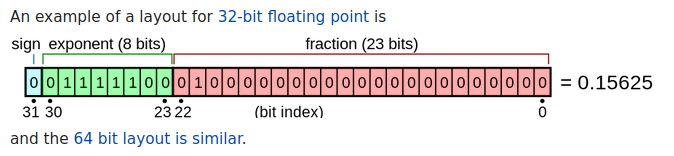
\includegraphics[width=0.8\textwidth]{figures/ieee754_1.png}
    \caption{An example taken from Wikipedia}
    \label{fig:figures-ieee754_1-png}
\end{figure}

So, essentially your real line has been discretized.

\subsection*{Quantization Error}
Given any $x \in  \R$ the computer takes it as $\hat{x}:=fl(x)$,
i.e. converts it to a floating point representation in its word
length.

\begin{equation}
    \hat{x} = \text{fl}(x) = x(1+\epsilon)
\end{equation}

$\epsilon$ is called the per-unit error.

What is the maximum possible error introduced when
converting a real quantity from $\R$ to IEEE 754? It's the
machine epsilon. Assume that the mantissa has $s$ bits. The
machine epsilon is given by
\begin{equation}
    u \approx \frac{1}{2}10^{1-s}
\end{equation}

\subsection*{Operations on Floating Point Numbers}
If you have a binary operator that works with two numbers
from $\R$, you want to be able to simulate it.

Let the `real' operation be $O(x,y)$, where  $x, y \in  \R$.
What the machine sees and does is $F(O(\hat{x},\hat{y}))$,
i.e. some errors will be introduced.
\begin{equation}
    \label{fpop}
    \begin{split}
        R &= F(O(x(1 + \epsilon_1), y(1 + \epsilon_2)))\\
          &= O(x,y)(1 + \epsilon)
    \end{split}
\end{equation}

Let's start with looking at what happens to our basic
arithmetic operations.

\subsubsection*{Multiplication}
\begin{equation}
    \begin{split}
        F(x_1x_2) &= (x_1(1+\epsilon_1)x_2(1 + \epsilon_2))(1 + \epsilon_3)\\
                  &= x_1x_2(1 + \epsilon_1)(1+\epsilon_2)(1+\epsilon_3)\\
                  &= x_1x_2(1 + \epsilon_1 + \epsilon_2
                  + \epsilon_3 + \mathcal{O}(u^3))
    \end{split}
\end{equation}
So, for multiplication the significant error goes as $3u\approx \mathcal{O(u)}$

\subsubsection*{Division}
\begin{equation}
F(\frac{x_1}{x_2}) \approx (\frac{x}{y})(1 + \varepsilon + \mathcal{O}(u^2))
\end{equation}

\subsubsection*{Addition}
This is troublesome
\begin{equation}
    \begin{split}
    F(x_1 + x_2) &= x_1(1 + \epsilon_1) + x_2(1 + \epsilon_2)\\
                 &= (x_1+x_2)(1 + \frac{x_1\epsilon_1}{x_1 + x_2} + \frac{x_2\epsilon_2}{x_1 + x_2})
    \end{split}
\end{equation}
The relative error depends on the operands. So, the error
will blow up if $x + y$ is small. This would happen if
$x$ and $y$ have similar magnitudes, different signs.

E.g. if $x = 1.24456$ and  $y = 1.23421$, so that
 $\hat{x} = 1.2346$ and $\hat{y} = 1.2342$. We have
$\hat{x} - \hat{y} = 0.0004$, while $x - y = 0.00035$.
This is like approximating 35 as 40. 14\% error.
Meanwhile, the truncation errors were some 0.001\%.
Absolutely mad.

This is called catastrophic cancellation.
This error can reach as high as 30\%. Imagine how much
error is introduced in Gaussian elimination. Computer
scientists were aware of the catastrophic cancellation
errors.

The only way around this is to use different numerical
algorithms, i.e. something that uses addition instead of
subtraction, and figure out the upper bounds for errors
in any numerical algorithm before we even start doing
the computation.
